\documentclass[12pt]{article}
\usepackage{graphicx}
\usepackage{amsmath}
\usepackage{geometry}
\usepackage{listings}
\usepackage{color}
\usepackage{array}
\usepackage{hyperref}
\usepackage{url}

\geometry{a4paper, margin=1in}

\definecolor{mygreen}{rgb}{0,0.6,0}
\definecolor{mygray}{rgb}{0.5,0.5,0.5}
\definecolor{mymauve}{rgb}{0.58,0,0.82}

\lstset{
	language=C++,
	basicstyle=\ttfamily\small,
	numbers=left,
	numberstyle=\tiny,
	stepnumber=1,
	numbersep=10pt,
	tabsize=4,
	breaklines=true,
	captionpos=b,
	keywordstyle=\color{blue}\bfseries,
	commentstyle=\color{mygray},
	stringstyle=\color{red}
}

\begin{document}
	\begin{titlepage}
		\centering
		
		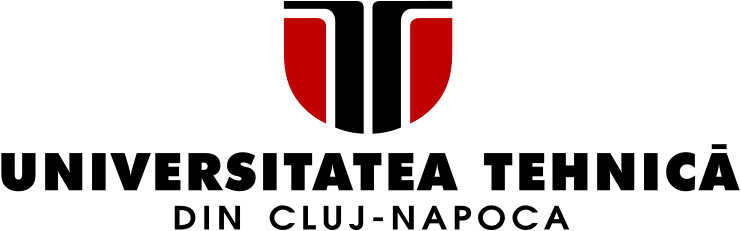
\includegraphics[width=0.4\textwidth]{Resources/logo_utcn.png}\\
		\vspace*{6cm}
		
		\Huge
		\textbf{Rendering a Minecraft Scene}
		
		\vspace{0.5cm}
		\Large
		Project Documentation
		
		\vspace{1.5cm}
		
		\textbf{Grad Laurentiu-Calin}\\
		\text{Group 30435}
		
		\vfill
		
		\Large
		Computer Science\\
		January, 2025\\
		
	\end{titlepage}
	
	\newpage
	
	\tableofcontents
	
	\newpage
	
	\section{Subject Specification}
	
	The purpose of this project is to design a scene and render it using OpenGL (with the help of the GLEW, GLFW and GLM extensions). Being an open-choice-themed scene, there were multiple implementation "paths" to pick from. The first one was to search the internet for open-source models, download them, import them into OpenGL and render them onto the screen. This download-and-paste method appeared to be a menace to me because 1. the models I found on the internet were not designed to be used with our project core configuration and 2. it is almost impossible to find open-source models that fit seamlessly (coherently) into a scene. Consequently, I decided to look for texures and map them myself onto objects using Blender. I am a Blender rookie so I looked for the simplest model I can texture: the default cube. This way the idea to design a Minecraft-related scene was born.
	
	For me, simulating the feeling of looking at Minecraft scenery is best described by the game-generated villages, so I decided to stick to this theme. The charm of a Minecraft village is a result of its composing structures: houses, churches, libraries, fountains, light poles made of torches, fences and wool etc. Creating some of these buildings became a core objective of the project.
	
	I did not look forward to implementing a one to one copy of a Minecraft village (I am particularly amazed by Minecraft shaders), meaning that I opted for a non-default, open-source texture pack. This is where all the textures I used came from. 
	
	\section{Scenario}
	\subsection{Scene \& Object Description}
	
	All the building/structures that are visible in the scene (except the land/floor/grass) are built from basic 2x2x2 blocks (or scaled versions, i.e. 2x4x2 for a door) created in Blender and exported as a pair (.obj, .mtl). This means each building is composed of between 20 up to 100 entities that are manually-placed level by level. 
	
	The scene is inspired from a default village generated in a taiga (spruce-tree-related) biome. The structures are made up by spruce logs and planks, cobblestone and stone bricks. When designing them I added a personal touch to their appearance (replaced cobblestone with planks or stone bricks, changed classic fences into morphed oak logs and so on).
	
	The scene takes place at night in a taiga village.  

	\subsection{Functionalities}
	
	\begin{enumerate}

		\item \textbf{camera movement} - any place in the scene can be reached by moving the camera accordingly; 

		\begin{itemize}
			\item \textbf{W} - move forward
			\item \textbf{A} - move left
			\item \textbf{S} - move backward
			\item \textbf{D} - move right
			\item \textbf{mouse/touchpad} - rotate the camera around all axis
			\item \textbf{scroll/pinch} - zoom in/out
		\end{itemize}

		\item \textbf{automated tour of the scene} - press \textit{1} to start an automated tour of the scene; during this process no input from outside (i.e. mouse, keyboard) is taken into account.		

		\item \textbf{toggle lighting} - press \textit{L} to toggle the light poles in the scene.
		
	\end{enumerate}
	
	\section{Implementation Details}
	
	\subsection{Functions \& Algorithms}
	
	\textbf{Functions \& Algorithms:} Explain the functions and algorithms used in your project.
	
	\subsubsection{Transparency}
	
	In order to make transparent elements (glass blocks, the windows in the door frame, the leaves), I had to sort them based on what direction I was facing. My implementation places all the objects to be rendered in a STL vector that is processed by the graphics pipeline. A thing to note is that the building blocks are added there without respect to the opacity. Consequently, after creating the scene, but before entering the game loop I had to separate them into transparent (glass, door, leaves) and non-transparent blocks (cobblestone, spruce and oak log, stairs etc). To do this I used a 2-pointer approach: i starts at the beginning and stops whenever it encounters a transparent block, j starts at the end and stops whenever it encounters a non-transparent block. When both of them stop I swap *i with *j. When i and j iterate over the entire array I stop. The final state of i is saved for further references.
		
	When I finish the above-mentioned process I solve 2 problems: I moved all the transparent blocks references in a contiguous memory location and I saved a pointer to the first element there. From now on, if I do not add new objects in the scene I know that all the objects I must sort to account for transparency are placed in the STL vector starting at position i up to the end.
		
	Finally, to account for transparency I must sort the transparent objects with respect to the direction the camera is facing. This means that in each iteration of the game loop I have to call a sort method on the ending part of the scene's object vector.
		
	\subsubsection{Possible Solutions}
	\textbf{Solutions:} Discuss the possible solutions you considered for implementing the project.
	
	\subsubsection{Motivation}
	\textbf{Motivation:} Explain the motivation behind your chosen solution.
	
	\subsection{Graphics Model}
	\textbf{Graphics Model:} Describe the graphical model used in your project.
	
	\subsection{Data Structures}
	\textbf{Data Structures:} List and explain the data structures used in your project.
	
	\subsection{Class Hierarchy}
	\textbf{Class Hierarchy:} Provide a diagram or description of the class hierarchy in your project.
	
	\section{Graphical User Interface Presentation}
	\textbf{GUI Presentation:} Present the graphical user interface of your project.
	
	\section{User Manual}
	\textbf{User Manual:} Provide instructions on how to use your project.
	
	\section{Conclusions}
	\textbf{Conclusion:}
	\begin{itemize}
		\item \textbf{Purpose Fulfillment:} Reflect on whether your project achieved its intended goals.
		\item \textbf{Potential Benefits:} Discuss how your solution can help others.
		\item \textbf{Practical Improvements:} Suggest ways in which the project could be improved.
	\end{itemize}
	
	\section{Further Developments}
	\textbf{Future Work:} Outline potential future developments and enhancements.
	
	\section{References}
	\textbf{References:} List all references and sources you used in your project. Use a proper citation style.
	
\end{document}
